\documentclass{beamer}
\mode<presentation>
\usetheme{Wisconsin}
\usepackage{times}
\usepackage{amsmath,amsthm,amssymb,latexsym,tikz}
\boldmath
\usepackage[english]{babel}
\usepackage[latin1]{inputenc}

\newcommand{\ZZ}{\mathbb{Z}}
\newcommand{\Acal}{\mathcal{A}}

%%%%%%%%%%%%%%%%%%%%%%%%%%%%%%%%%%%%%%%%%%%%%%%%%%%%%%%%%%%%%%%%%%%%%%%%%%%%%%%%%5
\title[LTO]{Link-Time Analysis to Optimize Library Usage}
\author[Chapman and He]{Mark Chapman and David He}
\institute[CS 706]{CS 706 Final Project}
\date[2010-12-08]{December 8, 2010}

%%%%%%%%%%%%%%%%%%%%%%%%%%%%%%%%%%%%%%%%%%%%%%%%%%%%%%%%%%%%%%%%%%%%%%%%%%%%%%%%%5
\begin{document}

\begin{frame}
  \titlepage
\end{frame}

\begin{frame}{Outline}
  \tableofcontents
\end{frame}

\section{Introduction}

\subsection{Motivation}

\begin{frame}{Problem}
  \begin{block}{Inefficient Library Usage}
    \begin{itemize}
    \item Authors: experts in field supply a module
    \item Users: application developers use modules
    \item {\it Problem:} optimal usage requires expertise by both parties
    \end{itemize}
  \end{block}
\pause
  \begin{block}{Separate the Concerns}
    \begin{itemize}
    \item Authors: supply insight to accomplish task {\bf efficiently}
    \item Users: supply logic to use library {\bf correctly}
    \item {\it Solution:} enable libraries to optimize themselves {\bf across method calls}, not just in separate calls
    \end{itemize}
  \end{block}
\end{frame}

\begin{frame}{Examples}
  \begin{block}{Rectangle}
    \begin{itemize}
    \item Need 4 values
      \begin{itemize}
      \item upper left x, upper left y, width, height
      \end{itemize}
    \item Remainder can be computed
      \begin{itemize}
      \item other corners x and y, center, height/width ratio
      \end{itemize}
\pause
    \item Look ahead and store {\bf only} values that are requested later
    \end{itemize}
  \end{block}
\pause
  \begin{block}{Data Structures}
    \begin{itemize}
    \item Map $\rightarrow$ HashMap or TreeMap
    \item List $\rightarrow$ LinkedList or ArrayList
    \item Only once use is known can the correct subtype be chosen
    \end{itemize}
  \end{block}
\end{frame}

\begin{frame}[fragile]
  \frametitle{Matrix Problem}
  \begin{semiverbatim}
  public static void main(String[] args) \{
    Matrix mA = MatrixFactory.create(
        new double[] \{\{1.0, 2.0\}, \{3.0, 4.0\}\});
    System.out.println(proc01(mA, 4));
  \}
  public static double[] proc01(Matrix mA, int k) \{
    \only<2->{mA = new EigenDecompMatrix(mA);}
    mA = MatrixOperations.power(mA, k);
    double[] vL = new double[mA.getNumRows()];
    MatrixOperations.eigenvalues(mA, vL);
    return vL;
  \}
  \end{semiverbatim}
\end{frame}

\subsection{Solution}

\begin{frame}{Overview}
  \begin{block}{Enforce Separation of Concerns}
    \begin{itemize}
    \item Library addresses performance internally
    \item Only abstract base types are visible to user
    \end{itemize}
  \end{block}
\pause
  \begin{block}{Optimize at Link-Time}
    \begin{itemize}
    \item Static analysis: flow sensitive, context insensitive
    \item Type flow: finds best types for list of method calls
    \item Insert transforms: convert between concrete types
    \end{itemize}
  \end{block}
\end{frame}

\section{Techniques}

\subsection{Implementation}

\begin{frame}{Implementation}
  \begin{block}{Link-Time Optimization (LTO)}
    \begin{itemize}
    \item Uses {\it java.lang.instrument} and {\it BCEL}
    \item Reads in annotations from self-optimizing library
    \item Transforms application bytecode when loaded
    \end{itemize}
  \end{block}
\pause
  \begin{block}{Library Information}
    \begin{itemize}
    \item {\it Manifest}: lists base types, methods, and transforms
    \item {\it @Equivalents}: annotations point base types to concrete subtypes and base methods (acting on base types) to called methods (acting on concrete types)
    \item {\it @Cost}: annotations give relative times for methods and transforms
    \end{itemize}
  \end{block}
\end{frame}

\subsection{Optimization}

\begin{frame}{Problem formulation}
  \begin{tabular}{rl}
  Variables &$X = x_1, x_2, \dotsc, x_{|X|}$ \\
  Types &$T = t_1, t_2, \dotsc, t_{|T|}$ \\
  Method calls &$M = m_1, m_2, \dotsc, m_{|M|}$
  \end{tabular}
  \vspace{0.5cm}

  A {\em configuration} is a type assignment of variables \[a : X \rightarrow T\]

  The set of all configurations is \[A = T^{X}\]
\end{frame}

\begin{frame}{Problem formulation}
  Cost of method calls \[CM: M \times A \rightarrow \ZZ\]
  Cost of type transforms \[CT: A \times A \rightarrow \ZZ\]

  Goal: Select $\Acal = a_1, a_2, \dotsc, a_{|M|}$ to minimize

  \[C(\Acal) = \sum_{i = 1}^{|M|} CM(m_i, a_i) + \sum_{i = 1}^{|M|} CT(a_{i - 1}, a_i).\]
\end{frame}

\begin{frame}{Network Flow}
  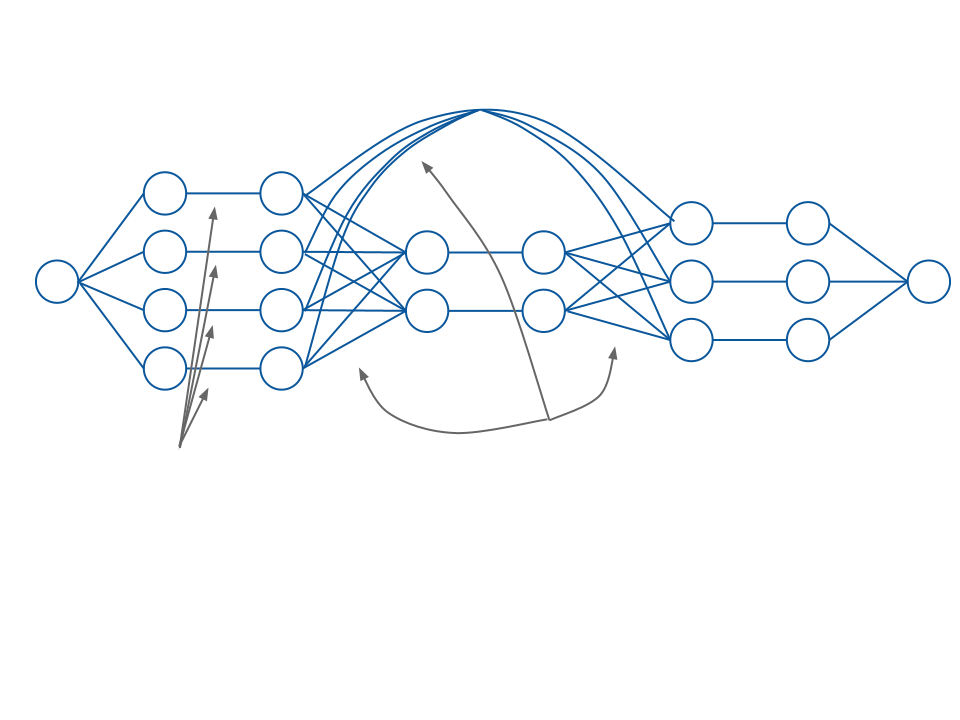
\includegraphics[scale=0.35]{cs706projflow}
\end{frame}

\begin{frame}{LP formulation}
  \begin{tabular}{lrl}
  directed graph $G = (V, E)$ & cost &$w: E \rightarrow \ZZ$ \\
  source $s$ sink $t$ & capacity &$c: E\rightarrow \ZZ$ \\
  flow $f$ &
  &
$ d(v) = 
  \begin{cases}
  f & \mbox{if } v=s\\
  -f & \mbox{if } v=t\\
  0 & \mbox{otherwise}
  \end{cases} 
  $
  \end{tabular}

  \uncover<2->{\alert<2>{$S_m = \{(v_{0ma}, v_{1ma}) \forall a\in A_m\}$}}
  \vspace{0.5cm}

  Minimize $\sum_{e\in E} w_e x_e$ subject to
  \begin{align*}
  \sum_{v : (v, u)\in E} x_{vu} - \sum_{v : (u, v)\in E} x_{uv} &= d(u) & \forall u \in V  \\
  x_e &\le c_e &\forall e \in E \\
  x_e &\ge 0 &\forall e \in E 
  \uncover<2->{\\x_e&\in \{0, f\} &\forall m, \forall e\in S_m}
  \end{align*}
\end{frame}

\section{Conclusion}

\subsection{Current Status}

\begin{frame}{Current Status}
  \begin{block}{Link-Time Analysis}
    \begin{itemize}
    \item Working pieces:
      \begin{itemize}
      \item reads manifest and annotations (from library)
      \item finds method calls (from application)
      \item optimizes over types
      \end{itemize}
    \item Remaining step: connect to optimizer to instrument application methods
    \end{itemize}
  \end{block}
\pause
  \begin{block}{Matrix Library}
    \begin{itemize}
    \item Limiting visibility to abstract base types makes some decisions difficult, e.g.\ user might want a {\it sparse} matrix
    \item Allow user to choose some type seeds or leave all decision to optimizer alone
    \end{itemize}
  \end{block}
\end{frame}

\subsection{Possible Future Work}

\begin{frame}{Possible Future Work}
  \begin{block}{Meaning of Cost}
    \begin{itemize}
    \item Annotate memory usage instead of execution time
    \item How could we annotate both and choose a balance?
    \end{itemize}
  \end{block}
\pause
  \begin{block}{Analysis}
    \begin{itemize}
    \item Static: add checkpoints where types may change
    \item Dynamic: change types depending on actual state
    \item Gains sensitivity to path and context
    \end{itemize}
  \end{block}
\pause
  \begin{block}{Type System}
    \begin{itemize}
    \item Qualifiers: finer control with lattice rather than hierarchy
    \item Multiple interfaces: alternative to positive qualifiers
    \end{itemize}
  \end{block}
\end{frame}

\end{document}
